%=======================================================================
%  Section 3 - PEFT: Text-to-LoRA (ICML 2025)
%   3.1 Bài toán   3.2 Liên quan   3.3 T2L (Module 1-4)   3.4 Thực nghiệm
%=======================================================================
\section{PEFT: Text-to-LoRA}

% ------------------------------------------------------------------ 3.1
\begin{frame}{3.1\quad Bài toán}{Khi có một tác vụ mới cần mô hình làm tốt}
  \Ask{Bạn sẽ làm gì? Fine-tune LoRA cho tác vụ mới --- và nếu đã có sẵn một số tác vụ rất giống thì sao?}

  \vspace{0.4em}
  \begin{columns}[T,onlytextwidth]
    \begin{column}{0.32\textwidth}
      \begin{beamercolorbox}[wd=\linewidth,sep=0.45em]{block body}
        \footnotesize\textbf{Nén các LoRA cũ bằng SVD}\\[0.15em]
        {\scriptsize\color{Muted}Tiết kiệm bộ nhớ, nhưng hiệu năng giảm.}
      \end{beamercolorbox}
    \end{column}
    \begin{column}{0.32\textwidth}
      \begin{beamercolorbox}[wd=\linewidth,sep=0.45em]{block body}
        \footnotesize\textbf{Chọn $k$ LoRA gần nhất}\\[0.15em]
        {\scriptsize\color{Muted}Bị giới hạn bởi các tác vụ cũ đã có.}
      \end{beamercolorbox}
    \end{column}
    \begin{column}{0.32\textwidth}
      \begin{beamercolorbox}[wd=\linewidth,sep=0.45em]{block alert body=AmberSoft,block alerted title}%
        \footnotesize\textbf{Dùng hypernetwork sinh adapter}\\[0.15em]
        {\scriptsize\color{Muted}Nhưng HN cũ nhận task-ID hoặc câu hỏi mẫu: bị giới hạn bởi tác vụ cũ, tốn train, và người dùng \emph{không kiểm soát} được.}
      \end{beamercolorbox}
    \end{column}
  \end{columns}

  \Takeaway{Mong muốn: \emph{một mô hình có thể sinh adapter từ chính mô tả của người dùng} --- không cần dữ liệu nhãn, không cần train lại.}
\end{frame}

% ------------------------------------------------------------------ 3.2
\begin{frame}{3.2\quad Công trình liên quan}{Hypernetwork}
  \begin{columns}[T,onlytextwidth]
    \begin{column}{0.47\textwidth}
      \justifying
      \textbf{Hypernetwork} là một mạng \emph{sinh ra trọng số} cho một mạng khác
      $W_l = h_\theta(\phi_l)$, với $\phi_l$ là mô tả của layer $l$
      (one-hot hoặc vector học được).

      \vspace{0.4em}
      Ý tưởng áp vào PEFT: thay vì sinh cả $W$ ($N\times N$), sinh các
      \emph{ma trận adapter} LoRA hạng thấp $\Delta W = BA$.
    \end{column}
    \begin{column}{0.47\textwidth}
      \centering
      \begin{tikzpicture}[font=\scriptsize, node distance=0.22cm,
          b/.style={draw=Navy, fill=Panel, rounded corners=2pt, minimum height=0.8cm, text width=2.5cm, align=center}]
        \node[b] (phi) {descriptor $\phi_l$};
        \node[b, fill=Navy, text=white, below=of phi] (h) {hypernetwork $h_\theta$};
        \node[b, below=of h] (w) {$W_l$ ($N\times N$)};
        \draw[-{Stealth}] (phi)--(h); \draw[-{Stealth}] (h)--(w);
        \node[right=0.15cm of w, text=Red!60!black, font=\tiny, text width=1.5cm, align=left] {quá lớn: $N^2$};
      \end{tikzpicture}\\[0.5em]
      \begin{tikzpicture}[font=\scriptsize, node distance=0.22cm,
          b/.style={draw=Navy, fill=Panel, rounded corners=2pt, minimum height=0.8cm, text width=2.5cm, align=center}]
        \node[b] (z) {mô tả tác vụ $z$};
        \node[b, fill=Navy, text=white, below=of z] (h2) {hypernetwork $h_\theta$};
        \node[b, below=of h2] (ab) {$A\in\mathbb{R}^{r\times d}$, $B\in\mathbb{R}^{d\times r}$};
        \draw[-{Stealth}] (z)--(h2); \draw[-{Stealth}] (h2)--(ab);
        \node[right=0.15cm of ab, text=PaperGreen, font=\tiny, text width=1.5cm, align=left] {nhỏ: $2rd$};
      \end{tikzpicture}
    \end{column}
  \end{columns}
  \Takeaway{Bước chuyển chính: đầu vào hypernetwork từ \emph{ID / câu hỏi mẫu} sang \emph{văn bản mô tả} --- thứ người dùng viết được.}
\end{frame}

% ------------------------------------------------------------------ 3.3
\begin{frame}{3.3\quad Text-to-LoRA}{Một mô hình sinh adapter từ mô tả}
  \begin{columns}[T,onlytextwidth]
    \begin{column}{0.46\textwidth}
      \justifying\footnotesize
      Khi có một tác vụ mới, T2L dùng \textbf{mô tả tác vụ} (trong paper do
      GPT-4o-mini sinh) làm đầu vào cho hypernetwork, từ đó sinh ra các ma trận
      adapter cho mô hình ngôn ngữ.

      \vspace{0.5em}
      \begin{beamercolorbox}[wd=\linewidth,sep=0.5em]{block body}
        \footnotesize
        \textbf{Một lượt chạy xuôi} $\rightarrow$ một bộ LoRA hoàn chỉnh.
        Không gradient, không dữ liệu nhãn, không chờ train.
      \end{beamercolorbox}
    \end{column}
    \begin{column}{0.5\textwidth}
      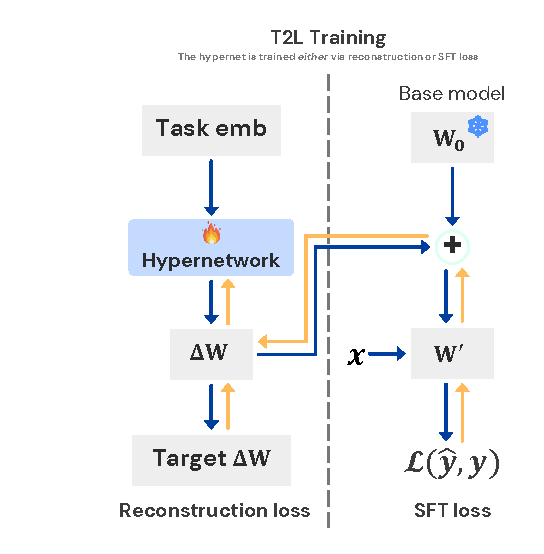
\includegraphics[width=\linewidth,height=0.47\textheight,keepaspectratio]{figure/t2l/fig1_train}%
      \par\vspace{0.2em}{\color{Muted}\scriptsize Fig 1 (trái): huấn luyện T2L --- tối ưu bằng reconstruction hoặc SFT.}
    \end{column}
  \end{columns}
\end{frame}

\begin{frame}{3.3\quad Module 1 --- Kiến trúc}{Architecture L / M / S}
  \FigureFull[0.42]{t2l/fig2_arch}{Fig 2: biến thể kiến trúc của T2L. Hộp xanh là module trainable, hộp cyan là embedding trainable; $r$ là hạng LoRA, $d$ là chiều ẩn.}
  \begin{columns}[T,onlytextwidth]
    \begin{column}{0.63\textwidth}
      \small
      \[
        \Delta W_{m,l}=h_\theta\!\left(\operatorname{concat}\big[f(z),\,E[m],\,E[l]\big]\right)
      \]
      \footnotesize\justifying
      $z$: mô tả tác vụ, $f$: text encoder, $E[m]$: loại module (key/value),
      $E[l]$: chỉ số layer.
    \end{column}
    \begin{column}{0.33\textwidth}
      \footnotesize
      Thêm $E[m]$ và $E[l]$ làm đầu vào là để \emph{một} bộ trọng số hypernetwork
      sinh được adapter cho mọi layer, mọi module.
    \end{column}
  \end{columns}
\end{frame}

\begin{frame}{3.3\quad Module 1 --- Cùng lúc sinh nhiều cặp (A,B)}
  \begin{columns}[T,onlytextwidth]
    \begin{column}{0.48\textwidth}
      \textbf{Vấn đề:} lớp FC đầu ra của hypernetwork sẽ khổng lồ nếu sinh cả $W$
      ($N\times N$). Chuyển sang một cặp $(A,B)$ kiểu LoRA đã nhỏ hơn nhiều ---
      nhưng Mistral-7B có 32 layer transformer $\Rightarrow$ cần một bộ adapter cho
      mỗi layer và mỗi module.

      \vspace{0.4em}
      Với hidden cuối $=512$, sinh đủ cho 7B bằng một lần sẽ cần
      $\approx 1.7$ tỉ tham số đầu ra.
    \end{column}
    \begin{column}{0.48\textwidth}
      \textbf{Cách của T2L:} thêm hai thuộc tính làm input ---
      \emph{layer thứ mấy} và \emph{module key hay value} --- rồi
      \textbf{chạy hypernetwork theo batch} cho mọi $(m,l)$ cùng lúc.

      \vspace{0.4em}
      Vì một lượt chạy chỉ mất vài chục mili giây, chạy 64 lần cho 64 cặp $(A,B)$
      vẫn nhanh hơn nhiều so với train LoRA.
    \end{column}
  \end{columns}
  \vspace{0.5em}
  \Takeaway{Chi phí tham số giảm từ $\sim$1.7B xuống $\sim$55M, còn thời gian vẫn tính bằng phần trăm giây.}
\end{frame}

\begin{frame}{3.3\quad Module 1 --- Ba mức đầu ra: L, M, S}
  \begin{columns}[T,onlytextwidth]
    \begin{column}{0.56\textwidth}
      \noindent\resizebox{\linewidth}{!}{%
      \small
      \setlength{\tabcolsep}{5pt}
      \begin{tabular}{@{}l l l c r@{}}
        \toprule
        Biến thể & Đầu ra & Input thêm & Batch & Tham số \\
        \midrule
        \textbf{L} & cả $A$ và $B$ & --- & 64 & $\sim$55M \\
        \textbf{M} & $A$ \emph{hoặc} $B$ & A/B emb & 128 & $\sim$34M \\
        \textbf{S} & một \emph{hàng} của $A$/$B$ & A/B $+$ rank emb & 1024 & $\sim$5M \\
        \bottomrule
      \end{tabular}}\\[0.4em]
      {\scriptsize\color{Muted}Ba biến thể đổi output kích thước lớn thành nhiều lần chạy nhỏ.}
    \end{column}
    \begin{column}{0.4\textwidth}
      \centering
      \begin{tikzpicture}[font=\scriptsize]
        \foreach \i/\n/\p/\c in {1/S/5/15, 2/M/34/45, 3/L/55/75}{%
          \pgfmathsetmacro{\bh}{\p/12}
          \fill[Navy!\c] (\i-0.38,0) rectangle (\i+0.38,\bh);
          \node[above, font=\scriptsize] at (\i,\bh) {\textbf{\n}};
          \node[below, font=\scriptsize, text=Muted] at (\i,0) {\p M};
        }
        \draw[Muted] (0.4,0) -- (3.6,0);
        \node[font=\scriptsize, text=Muted] at (2,2.1) {tham số đầu ra};
      \end{tikzpicture}
    \end{column}
  \end{columns}
  \Takeaway{Không phải chọn một: paper cho thấy cả ba đều cạnh tranh, và S nhẹ nhất lại mạnh nhất trên một số tác vụ (PIQA).}
\end{frame}

\begin{frame}{3.3\quad Module 2 --- Độ nhạy với mô tả}{Cùng một bài toán, ba mô tả}
  \begin{columns}[T,onlytextwidth]
    \begin{column}{0.5\textwidth}
      {\footnotesize\color{Muted}Toulouse has twice as many sheep as Charleston. Charleston has 4 times as many sheep as Seattle. How many sheep do Toulouse, Charleston, and Seattle have together if Seattle has 20 sheep?}

      \vspace{0.25em}
      \begin{itemize}\tightlist\footnotesize
        \item \textbf{(i)} Mô hình gốc: giải đúng từng bước, CoT dài;
        \item \textbf{(ii)} Mô tả chất lượng kém \emph{“solve this task please”}:
              vẫn ra 240, nhưng rất ngắn;
        \item \textbf{(iii)} Mô tả thiên toán học: suy luận trực tiếp hơn, nhưng
              \emph{tính sai} ($260$);
        \item \textbf{(iv)} Mô tả thiên lập trình: tiếp cận thuật toán từng bước.
      \end{itemize}
    \end{column}
    \begin{column}{0.47\textwidth}
      \FigureFull[0.62]{t2l/fig4_qualitative}{Fig 4: cùng một câu hỏi, LoRA sinh từ bốn mô tả khác nhau cho bốn phong cách trả lời khác nhau.}
    \end{column}
  \end{columns}
  \Takeaway{LoRA sinh ra \emph{steerable}: đổi mô tả là đổi hành vi --- nhưng vẫn có thể sai (như ví dụ iii).}
\end{frame}

\begin{frame}{3.3\quad Module 3 --- Text encoder}{Tại sao dùng encoder ngoài, và tại sao là gte-large-en}
  \begin{columns}[T,onlytextwidth]
    \begin{column}{0.48\textwidth}
      \begin{beamercolorbox}[wd=\linewidth,sep=0.55em]{block title}
        \centering Tại sao không dùng encoder của LM?
      \end{beamercolorbox}
      \vspace{0.3em}
      \footnotesize\justifying
      Encoder của LM đã được huấn luyện cho \emph{mục tiêu khác} (dự đoán token).
      Paper dẫn lập luận của HINT và HyperTune: một text encoder \emph{độc lập},
      chuyên cho biểu diễn câu, cho embedding mô tả tốt hơn --- và giữ LM không
      phải sửa.
    \end{column}
    \begin{column}{0.48\textwidth}
      \begin{beamercolorbox}[wd=\linewidth,sep=0.55em]{block title}
        \centering Vì sao là gte-large-en-v1.5?
      \end{beamercolorbox}
      \vspace{0.3em}
      \footnotesize\justifying
      Tại thời điểm viết paper (2025), đây là một trong những encoder nhỏ mạnh nhất
      ở nhiệm vụ embedding câu, chỉ $\sim$400M tham số --- đủ nhẹ để chạy cạnh
      hypernetwork.

      \vspace{0.3em}
      T2L dùng activation của token CLS ở layer cuối (model là bidirectional).
    \end{column}
  \end{columns}
  \vspace{0.4em}
  \Takeaway{Đọc kỹ: encoder \emph{không} phải thứ được train trong SFT --- hypernetwork mới là thứ học.}
\end{frame}

\begin{frame}{3.3\quad Module 4 --- Hai cách train hypernetwork}
  \begin{columns}[T,onlytextwidth]
    \begin{column}{0.48\textwidth}
      \begin{beamercolorbox}[wd=\linewidth,sep=0.55em]{block title}
        \centering Reconstruction
      \end{beamercolorbox}
      \vspace{0.3em}
      \footnotesize\justifying
      \begin{enumerate}\tightlist
        \item Train sẵn LoRA riêng cho \emph{từng} tác vụ trong thư viện;
        \item Hypernetwork sinh adapter, so với adapter thật bằng MSE;
        \item Cập nhật hypernetwork.
      \end{enumerate}
      {\scriptsize\color{Muted}Cần trước một thư viện LoRA đã train.}
    \end{column}
    \begin{column}{0.48\textwidth}
      \begin{beamercolorbox}[wd=\linewidth,sep=0.55em]{block title}
        \centering SFT
      \end{beamercolorbox}
      \vspace{0.3em}
      \footnotesize\justifying
      \begin{enumerate}\tightlist
        \item Hypernetwork sinh adapter;
        \item Gắn adapter vào LM \emph{đóng băng} để trả lời câu hỏi;
        \item Dùng cross-entropy của câu trả lời để cập nhật hypernetwork.
      \end{enumerate}
      {\scriptsize\color{Muted}Học end-to-end trên tác vụ thật.}
    \end{column}
  \end{columns}
  \vspace{0.4em}
  \Takeaway{Reconstruction học “chép” trọng số; SFT học “làm đúng việc” --- và paper cho thấy khác biệt lớn.}
\end{frame}

\begin{frame}{3.3\quad Module 4 --- Reconstruction vs SFT}
  \begin{columns}[T,onlytextwidth]
    \begin{column}{0.5\textwidth}
      \centering\footnotesize
      \begin{tabular}{@{}lccc c@{}}
        \toprule
        & \multicolumn{3}{c}{Benchmark} & \\
        \cmidrule(lr){2-4}
        & S & M & L & TB \\
        \midrule
        Reconstruction & 61.8 & 61.7 & 62.0 & 61.8 \\
        \textbf{SFT}   & 64.8 & 66.5 & \Win{67.5} & \Win{66.3} \\
        \bottomrule
      \end{tabular}\\[0.5em]
      {\scriptsize\color{Muted}Bảng 6: cùng khoảng thời gian train ($\sim$10 giờ) cho mỗi cấu hình.}
    \end{column}
    \begin{column}{0.46\textwidth}
      \textbf{Tại sao SFT thắng?}
      \begin{itemize}\tightlist\footnotesize
        \item Hai bộ trọng số khác nhau có thể cho cùng hành vi
              $\Rightarrow$ \emph{không đồng nhất nghiệm tối ưu} của MSE;
        \item MSE đo khoảng cách trọng số, \emph{không} đo độ tốt của mô hình;
        \item SFT bỏ được yêu cầu thư viện LoRA: học trực tiếp từ mục tiêu cuối.
      \end{itemize}
    \end{column}
  \end{columns}
  \vspace{0.3em}
  \Takeaway{Đây là lập luận cốt lõi của paper: mục tiêu cuối là \emph{trả lời đúng}, nên loss phải đo điều đó.}
\end{frame}

% ------------------------------------------------------------------ 3.4
\begin{frame}{3.4\quad Thực nghiệm}{So với task-specific LoRA (9 tác vụ đã thấy khi train)}
  \begin{columns}[T,onlytextwidth]
    \begin{column}{0.66\textwidth}
      \centering
      \resizebox{\linewidth}{!}{%
      \scriptsize
      \begin{tabular}{@{}l ccccccccc c@{}}
        \toprule
        & ArcC & ArcE & BQ & GSM8K & HS & OQA & PIQA & WG & MBPP & TB \\
        \midrule
        Base model              & 65.4 & 77.8 & 71.6 & 40.9 & 49.7 & 54.2 & 72.8 & 45.0 & 43.1 & 55.8 \\
        \midrule
        \multicolumn{11}{@{}l}{\scriptsize\color{Muted}One-hot task embedding} \\
        T2L (Recon) L           & \Win{76.4} & 89.9 & 89.4 & \Win{53.8} & 92.6 & 85.0 & 69.7 & 51.2 & 52.6 & \Win{73.4} \\
        T2L (Recon) M           & \Win{76.7} & 89.9 & 89.4 & 53.2 & 92.6 & 85.0 & 69.9 & 51.4 & 52.9 & \Win{73.4} \\
        T2L (Recon) S           & 75.2 & 88.8 & 87.4 & 50.9 & 89.1 & 75.6 & \Win{83.9} & \Win{58.1} & 48.1 & 73.0 \\
        \midrule
        \multicolumn{11}{@{}l}{\scriptsize\color{Muted}Task description embedding} \\
        T2L (Recon) L           & 76.6 & 89.8 & 89.4 & 53.9 & 92.6 & 85.0 & 69.6 & 51.2 & 51.8 & 73.3 \\
        T2L (Recon) M           & 76.5 & 89.9 & 89.4 & 53.9 & 92.5 & 84.9 & 70.4 & 51.6 & 52.8 & \Win{73.5} \\
        T2L (Recon) S           & 75.4 & 88.8 & 87.8 & 49.1 & 89.7 & 76.7 & \Win{84.2} & \Win{56.9} & 48.0 & 73.0 \\
        \midrule
        Task-specific LoRA (oracle) & 76.6 & 89.9 & 89.4 & 53.5 & 92.6 & 85.0 & 69.9 & 51.1 & 52.1 & 73.3 \\
        \bottomrule
      \end{tabular}}
    \end{column}
    \begin{column}{0.3\textwidth}
      \footnotesize\justifying
      T2L \textbf{khôi phục gần như hoàn toàn} hiệu năng LoRA oracle, và
      \textbf{vượt oracle} ở nhiều tác vụ.

      \vspace{0.4em}
      Lý do được paper đưa ra: nén \emph{lossy} đóng vai trò như
      regularization --- rõ nhất ở PIQA và WG, nơi oracle LoRA bị overfit.
    \end{column}
  \end{columns}
\end{frame}

\begin{frame}{3.4\quad Thực nghiệm}{Zero-shot trên tác vụ \emph{chưa} thấy khi train}
  \begin{columns}[T,onlytextwidth]
    \begin{column}{0.6\textwidth}
      \centering
      \resizebox{\linewidth}{!}{%
      \scriptsize
      \begin{tabular}{@{}l cccccccc c cc c@{}}
        \toprule
        & ArcC & ArcE & BQ & HS & OQA & PIQA & WG & MBPP & TB(8) & GSM8K & HE & TB(10) \\
        \midrule
        No test-time adaptation \\
        \quad Mistral-7B-Instruct & 65.4 & 77.8 & 71.6 & 49.7 & 54.2 & 72.8 & 45.0 & 43.1 & 60.0 & 40.9 & 37.2 & 55.8 \\
        \quad Prepending task desc. & 72.0 & 85.8 & 67.6 & 58.9 & 63.4 & 77.9 & 59.0 & 41.6 & 65.8 & 40.9 & 39.0 & 60.6 \\
        \quad 3-shot ICL & 72.1 & 85.9 & 71.7 & 59.0 & 66.2 & 76.2 & 58.0 & 42.6 & 66.5 & 40.9 & 37.2 & 61.0 \\
        \quad Multi-task LoRA & 76.2 & 88.3 & \Win{85.5} & 65.2 & 68.0 & 81.8 & 62.4 & 48.1 & 71.9 & 47.5 & 39.6 & 66.3 \\
        \midrule
        Zero-shot adaptation \\
        \quad Arrow Routing & 60.9 & 86.2 & 87.6 & 80.8 & 48.6 & 83.0 & 68.5 & \Win{50.2} & 70.7 & --- & 28.7 & --- \\
        \quad Hyperdecoders & \Win{76.6} & 88.5 & 83.9 & 65.2 & \Win{76.6} & 81.3 & 64.9 & 51.6 & \Win{73.6} & 43.6 & \Win{40.9} & 67.3 \\
        \quad T2L (SFT) S & 76.0 & 88.7 & 83.8 & \Win{68.0} & 71.6 & \Win{82.3} & 61.0 & 41.2 & 71.6 & \Win{47.3} & 39.0 & 65.9 \\
        \quad T2L (SFT) M & 77.2 & 89.0 & 84.3 & 65.1 & 76.1 & 81.8 & 64.0 & 50.5 & 73.5 & 45.2 & \Win{41.3} & 67.5 \\
        \quad \textbf{T2L (SFT) L} & \Win{77.5} & \Win{88.9} & 85.0 & 66.5 & 75.5 & 82.1 & 64.2 & 51.9 & \Win{73.9} & 45.8 & 39.2 & \Win{67.7} \\
        \bottomrule
      \end{tabular}}
    \end{column}
    \begin{column}{0.36\textwidth}
      \begin{itemize}\tightlist\footnotesize
        \item T2L \textbf{vượt multi-task LoRA} một cách nhất quán;
        \item Vượt cả oracle ở một số tác vụ;
        \item Chưa đóng hết khoảng cách với LoRA riêng từng tác vụ;
        \item Arrow Routing không sinh được adapter cho tác vụ quá xa.
      \end{itemize}
      \vspace{0.3em}
      {\scriptsize\color{Muted}Bảng 2 (rút gọn): TB(8) bỏ GSM8K và HumanEval, TB(10) gồm cả hai.}
    \end{column}
  \end{columns}
\end{frame}

\begin{frame}{3.4\quad Thực nghiệm}{T2L mở rộng tốt khi có nhiều tác vụ train hơn}
  \begin{columns}[T,onlytextwidth]
    \begin{column}{0.44\textwidth}
      \FigureFull[0.6]{t2l/fig1_scaling}{Fig 1 (phải): điểm zero-shot trên 10 benchmark khi tăng số tập dữ liệu pretrain.}
    \end{column}
    \begin{column}{0.5\textwidth}
      \begin{itemize}\tightlist\footnotesize
        \item Từ 64 lên 479 tác vụ, cả L/M/S đều tăng điểm;
        \item Trên 479 tác vụ: L đạt \textbf{67.7}, M 67.5, S 65.2;
        \item T2L vượt \textbf{MT-LoRA} --- baseline fine-tune multi-task thường;
        \item Nhưng vẫn sau oracle LoRA riêng cho từng tác vụ.
      \end{itemize}
      \vspace{0.3em}
      \FigureFull[0.26]{t2l/fig3_error}{Fig 3: điểm tương đối so với oracle giảm khi lỗi reconstruction tăng --- nén là \emph{lossy}.}
    \end{column}
  \end{columns}
\end{frame}
